\section{Digitaltechnik}

\subsection{Operatoren}
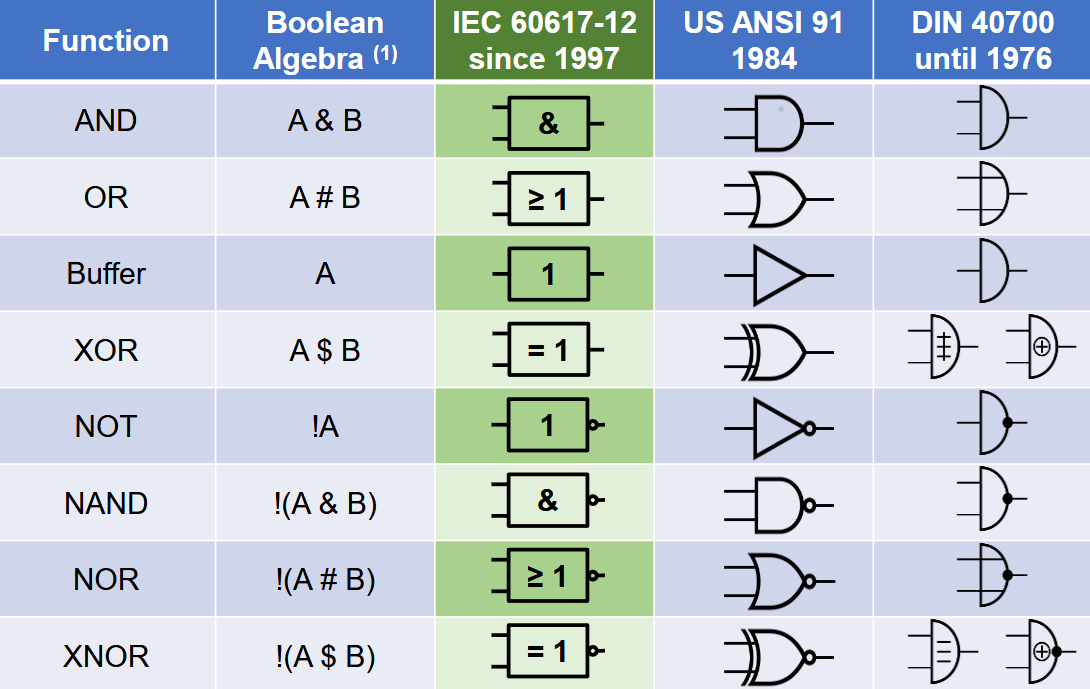
\includegraphics[scale=0.3]{img/symbols}
\subsection{Flip-Flops}
Flip-Flops sind Speicherelemente, die den Zustand speichern und bei einem Taktimpuls den Zustand ändern.
Ein normaler "D-Flip-Flop" kann genau ein Bit Information speichern.
\begin{itemize}
    \item Clock $C$
    \item Data $D$
    \item Ausgang $Q$
\end{itemize}

\begin{circuitikz}
    \node[flipflop DQ](ff1){};
  \end{circuitikz}